\section{Introduction}

La posturographie, aussi appelée posturologie est une technique employée pour évaluer,
mesurer et contrôler la posture en position debout.

Pour maintenir un équilibre vertical, le corps humain ajuste en permanence sa posture par rapport 
à son environnement en fonction de certains signaux qu'il reçoit. Ces signaux sont captés par les yeux, la colonne vertébrale, 
l'oreille interne ou encore les pieds. Le cerveau les analyse et envoie des instructions au corps dans le but de modifier 
sa posture en temps réel aux différents éléments perçus.

Si ces signaux, importants pour le maintien de l'équilibre ne sont pas ou mal perçus, ou mal analysés, la posture ne sera pas 
correctement adaptée, et des troubles tels que des déséquilibres, des vertiges ou encore des problèmes \textit{musculosquelettiques} 
pouvant aller jusqu'à des douleurs chroniques dans certaines régions de l'organisme pourraient apparaître.

Il est donc important pour les posturologues de mettre aujourd'hui l'accent sur l'étude du rôle des yeux, des pieds ainsi que les occlusions dentaires 
dans les problèmes liées à la posture.

Cette discipline étudie la position de l’homme dans l’espace (son équilibre,
sa stature, son aplomb, sa stabilité...) grâce à des appareils de mesure spécialisés.
Elle prend en compte la capacité de rester en équilibre sur ses pieds ainsi que la
symétrie du corps ou la perception visuelle de l’horizontalité. 

Ces études sont possibles aussi bien dans des situations
\textbf{statiques} que \textbf{dynamiques}.

\subsection{Posturographie dynamique}

La posturographie dynamique informatisée (aussi appelée \textit{Test of Balance}) est une technique d'évaluation clinique non invasive. 
Cette méthode permet de mesurer et quantifier les mécanismes d'adaptation du système nerveux central intervenant dans le contrôle de la posture et de l'équilibre d'un patient \textbf{en mouvement}.

Ces mécanismes interviennent aussi bien dans des conditions dites normales (comme pendant des entrainements sportifs), que dans des conditions dites anormales, notamment lors du diagnostic de troubles d'équilibre, de la physiothérapie ou de la rééducation posturale.

La posturographie dynamique informatisée (CDP) exige différents protocoles.
En effet, les interactions entre les différents agents du corps impliquées dans la posture et l’équilibre sont complexes.
Ces protocoles permettent de faire la distinction entre les nombreux problèmes et limitations influençant les système de régulation postural du patient.

\begin{figure}[ht]
    \centering
    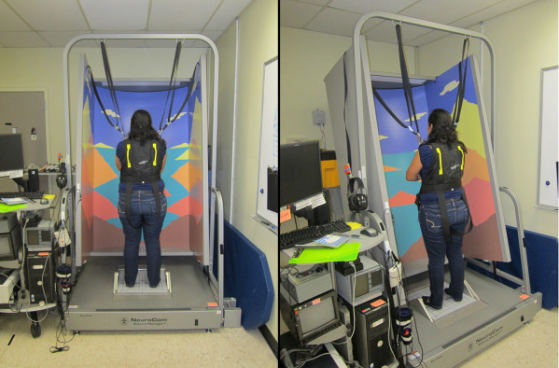
\includegraphics[width=0.5\textwidth]{images/introduction/dynamique.png}
    \caption{Posturographie dynamique}
    \label{fig:posturographie-dynamique}
\end{figure}

\subsection{Posturographie statique}

La posturographie statique évalue quant à elle la posture d'un patient en \textit{équilibre orthostatique} \\ (position érigée immobile, fondamentale de l'espèce humaine).
Cette évaluation se fait en positionnant le patient sur une plateforme équipée de nombreux capteurs de pression.

L'enregistrement des oscillations du centre de pression des pieds permettent de retracer l'évolution du centre de gravité (ou centre de masse) du patient.

Lors de ces évaluations, on étudie aussi la réponse posturale du patient à certaines perturbations.

\begin{figure}[ht]
    \centering
    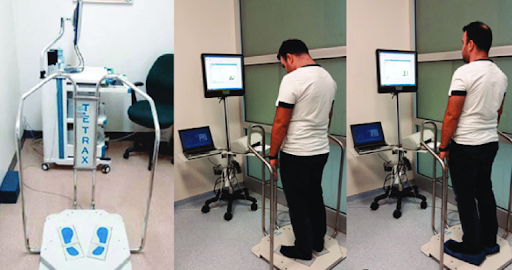
\includegraphics[width=0.5\textwidth]{images/introduction/statique.png}
    \caption{Posturographie statique}
    \label{fig:posturographie-statique}
\end{figure}